\documentclass[aspectratio=169]{beamer}

\usepackage{beamerthemesplit}
\usepackage{amsmath}
\usepackage{amsfonts}
\usepackage{amssymb}
\usepackage{cancel}
\usepackage{bussproofs}
%% \usepackage{tkz-graph}

\makeatletter
\newcommand{\reallytiny}{\@setfontsize{\srcsize}{2pt}{2pt}}
\makeatother

\mode<presentation>
{
  \usetheme{AnnArbor}
  \usecolortheme{crane}
}

\usepackage[english]{babel}
\usepackage[latin1]{inputenc}
\usepackage{times}
\usepackage[T1]{fontenc}

\title{AGI-20 Tutorial\\ OpenCog, PLN and Pattern Miner}

\author{Nil Geisweiller, Matt Ikle}

\institute[SingularityNET OpenCog Foundations]
{
  \begin{center}
    SingularityNET \& OpenCog Foundations\\
    
\includegraphics[scale=0.32]{images/snet_oc.png}
  \end{center}
}
          
\date[AGI-20]

\begin{document}

\begin{frame}
  %% It's gonna be a tutorial mainly focused on reasoning using
  %% OpenCog, although as you'll see it's actually quite broad as that
  %% includes some forms of learning, such as pattern mining, which
  %% we'll go over as well.

  \maketitle
\end{frame}

\section {Preparation}

\begin{frame}
  %% Because there's a docker image to download for this tutorial,
  %% we're going to take care of that first, and while it's
  %% downloading in the background I'll give a short introduction to
  %% OpenCog and what we're gonna cover.

  %% \frametitle{Preparation}
  \begin{enumerate}
  \item Install docker
    \begin{itemize}
    \item Debian/Ubuntu
      \begin{semiverbatim}sudo apt install docker.io\end{semiverbatim}
      \item Arch/Manjaro
        \begin{semiverbatim}sudo pacman -S docker\end{semiverbatim}
    \end{itemize}
  \item Download docker image (1.6GB)
    \begin{semiverbatim}sudo docker pull ngeiswei/opencog:agi20\end{semiverbatim}      
  \end{enumerate}
\end{frame}

\section {OpenCog}

\begin{frame}
  %% OpenCog is a framework for doing AGI research and solve real
  %% problems as well.  It's been used for many things such as
  %% controlling virtual or real agents, for bio-informatics, the list
  %% is long.

  %% What it offers are

  %% 1. A hypergraph database, call the AtomSpace with a language,
  %%    called Atomese, to query, rewrite and generally operate over
  %%    the atomspace.

  %% 2. Cognitive processes, called Mind Agents, for reasoning (that's
  %%    what we'll focus on here), learning, making decision, natural
  %%    language processing, and more things, such as what Alexey
  %%    Potapov and his team are working on, and that they will have a
  %%    chance to present during the conference.

  %% \frametitle{OpenCog}

  \center{Framework for AGI}\\[0.5cm]

  \begin{columns}
    \column{3in}
  
    \begin{enumerate}
    \item Hypergraph Database: 
      \begin{itemize}
      \item AtomSpace
      \item Atomese: query, rewrite and more
      \end{itemize}
    \item Mind Agents (cognitive processes):
      \begin{itemize}
      \item \alert{Reasoning: PLN, Miner}
      \item Learning: MOSES, Miner
      \item Decision: OpenPsi (Bach's MicroPsi)
      \item Language Processing
      \item Attention Allocation
      \end{itemize}
    \end{enumerate}

    \column{3in}

    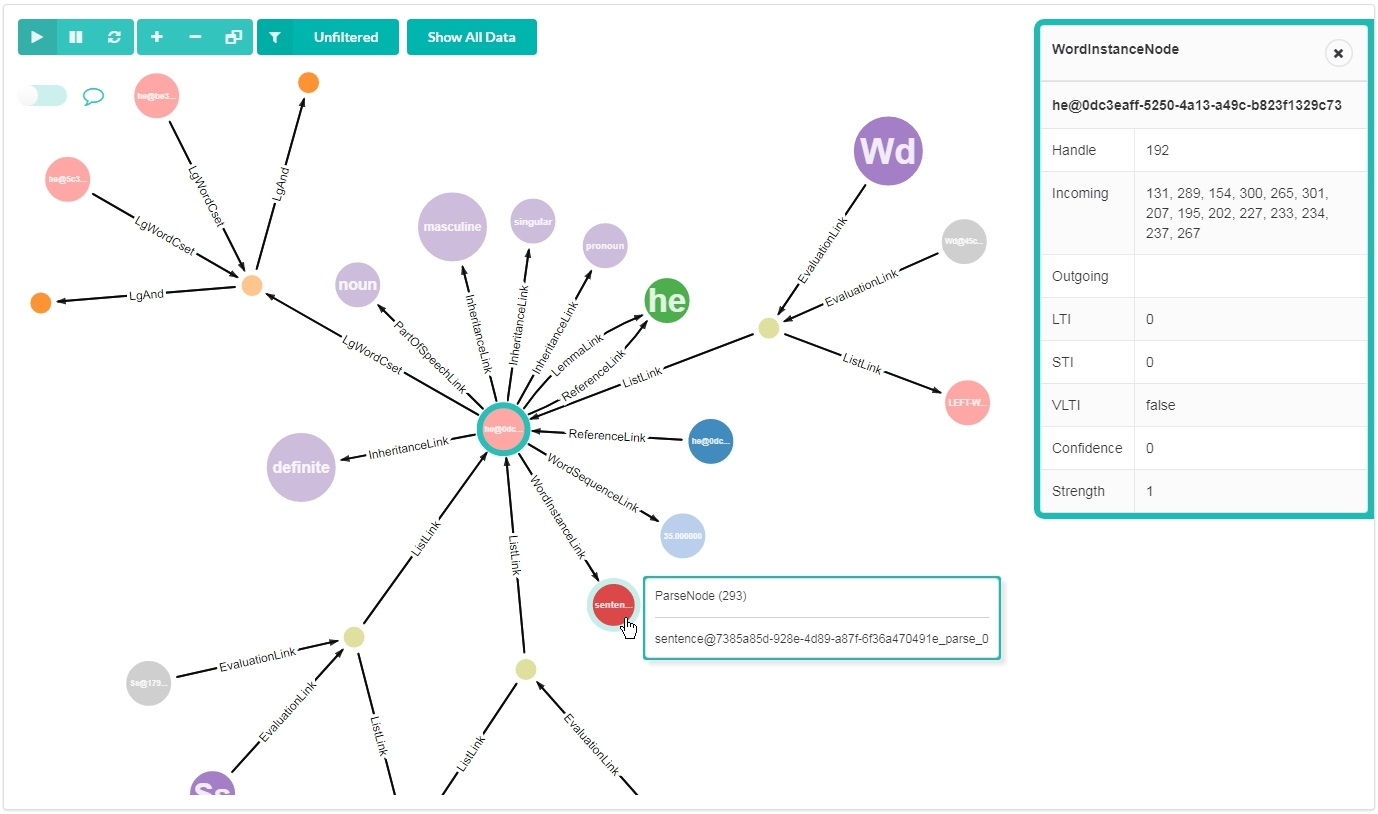
\includegraphics[scale=0.2]{images/ng2-atomspace-visualizer.jpg}

  \end{columns}

  - - - - - - - - - - - - - - - - - - - - - - - - - - - - - - - - - -
  - - - - - - - - - - - - - - - - - - - - - - - - - - - - - - - - -\\[0.1cm]
  \center{Download docker image: \texttt{\textcolor{black}{sudo docker pull ngeiswei/opencog:agi20}}}

\end{frame}

\section {PLN}

\begin{frame}
  %% I'm gonna give a quit presentation of what is PLN, which should
  %% help you to understand what is going on during the tutorial.

  %% PLN stands for Probabilistic Logic Network, it was invented by
  %% Ben, Matt and a few others. It was really created specifically
  %% for the AtomSpace, to handle common sense reasoning, and just
  %% about every type of reasoning that's useful for dealing with the
  %% king declarative knowledge that is stored in the AtomSpace (you
  %% may correct me Matt if I'm saying something inaccurate).

  %% It basically builds upon Probability Theory it to handle
  %% uncertainty (with a probabilistic semantics, I'll show that
  %% next), but it's also a logical system, more or less a super-set
  %% of predicate logic.  And although it's particularly well suited
  %% for common sense reasoning it can handle mathematical reasoning
  %% as well, like a theorem prover would, even though it's been
  %% rather under-explored so far.

  %% An important point about PLN and the way it's been used is that
  %% it can reason about its own resource management, therefore
  %% enabling a form of meta-reasoning, to improve its efficiency over
  %% time.

  %% \frametitle{PLN}

  \begin{columns}
    \column{2.5in}
    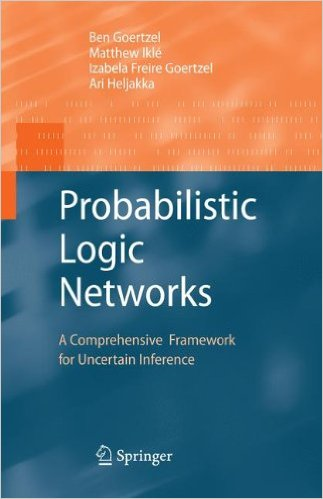
\includegraphics[scale=0.32]{images/PLN.jpg}\\

    \column{3in}
    \begin{itemize}
    \item Probability Theory
    \item Uncertainty management
    \item Common sense reasoning
    \item Mathematical reasoning
    \item Resource management
    \end{itemize}

  \end{columns}

  - - - - - - - - - - - - - - - - - - - - - - - - - - - - - - - - - -
  - - - - - - - - - - - - - - - - - - - - - - - - - - - - - - - - -\\[0.1cm]
  \center{Download docker image: \texttt{\textcolor{black}{sudo docker pull ngeiswei/opencog:agi20}}}

\end{frame}

\subsection {Basics}

\begin{frame}
  %% TODO
  
  %% Or rather an estimate of that probability.  And c is the
  %% confidence, defined with that formula.  The formula itself
  %% doesn't really matter, what matters is that we have a monotonic
  %% mapping between the size of A and the range zero one, so that as
  %% the size goes to infinity the confidence goes to one.

  %% OK, but why is that called simple truth value? Well, as you
  %% probably, it's because we also have more complex truth values,
  %% the reason is because underneath a truth value is a second order
  %% distribution.

  %% \frametitle{PLN: the basics}

  \begin{columns}
    \column{1in}
    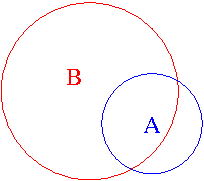
\includegraphics[scale=0.8]{images/subset_A_B.pdf}

    \column{2.7in}
\texttt{(Subset (stv s c)\\
\ \ \ \ A\\
\ \ \ \ B)}\\[0.22cm]

\begin{block}
  {Definitions:}
  {\begin{itemize}
    \item \texttt{stv} = \textit{Simple Truth Value}
    \item \texttt{Subset A B} = $P(B|A)$
    \item \texttt{s} = strength = $\displaystyle P(B|A)=\frac{|A \cap B|}{|A|}$
    \item \texttt{c} = confidence = $\displaystyle \frac{|A|}{|A| + K}$
    \end{itemize}}
\end{block}

  \end{columns}

  - - - - - - - - - - - - - - - - - - - - - - - - - - - - - - - - - -
  - - - - - - - - - - - - - - - - - - - - - - - - - - - - - - - - -\\[0.1cm]
  \center{Download docker image: \texttt{\textcolor{black}{sudo docker pull ngeiswei/opencog:agi20}}}

\end{frame}

\begin{frame}
  %% So basically when the confidence in null the second order
  %% distribution is flat if you use a Bayesian prior, or slightly
  %% concave is you use a Jeffrey prior, and as measure as the number
  %% of observations grow the second order distribution narrows down
  %% to a particular value. OK, but that's if you model the second
  %% order distribution with a beta-distribution, which is justified a
  %% lot of the time, but not always, if you start doing inference and
  %% aggregate data from different sources, that sort of things, a
  %% beta-distribution might no longer adequate.  A beta-distribution
  %% has two parameters so has a Simple Truth Value, a strength and a
  %% confidence, so it's enough for that case, but in general it's
  %% not, which is why we need more complex types of truth value than
  %% simple truth value.

  %% \frametitle{PLN: the basics}

  \center{\textit{Truth Value = \textcolor{red}{Second Order Distribution}}}\\[1.45cm]

  \begin{columns}
    \column{1.65in}
    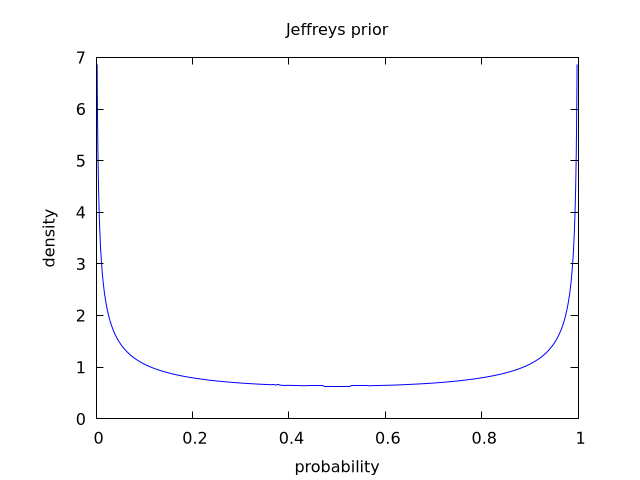
\includegraphics[scale=0.2]{images/jeffreys_prior.png}  

    \column{1.65in}
    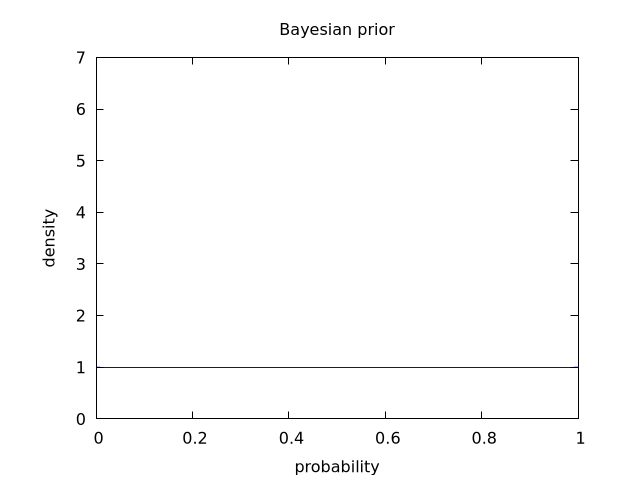
\includegraphics[scale=0.2]{images/bayesian_prior.png}  

    \column{1.65in}
    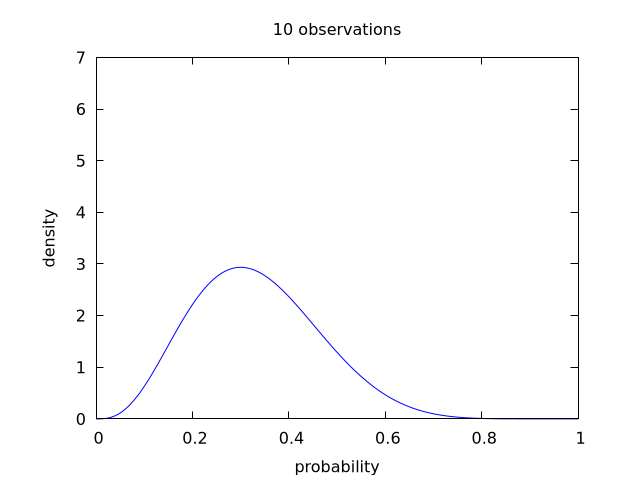
\includegraphics[scale=0.2]{images/observations_10.png}  

    \column{1.65in}
    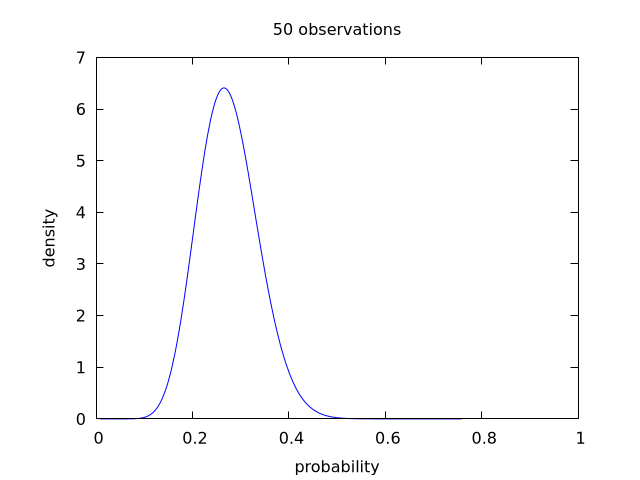
\includegraphics[scale=0.2]{images/observations_50.png}  
  \end{columns}

  - - - - - - - - - - - - - - - - - - - - - - - - - - - - - - - - - -
  - - - - - - - - - - - - - - - - - - - - - - - - - - - - - - - - -\\[0.1cm]
  \center{Download docker image: \texttt{\textcolor{black}{sudo docker pull ngeiswei/opencog:agi20}}}

\end{frame}

\subsection{Example}

\begin{frame}

  {\small
    \begin{itemize}
    \item Knowledge base:\\
      \texttt{(Subset (stv 0.4 0.1) A B)}\\
      \texttt{(Subset (stv 0.6 0.2) B C)}\\
      \texttt{A (stv 0.1 0.6)}

    \item Rule base:\\
      \begin{prooftree}
        \AxiomC{\texttt{(Subset <tv1> X Y)}}
        \AxiomC{\texttt{(Subset <tv2> Y Z)}}
        \RightLabel{(Deduction)}
        \BinaryInfC{\texttt{(Subset <tv3> X Z)}}
      \end{prooftree}

      \begin{prooftree}
        \AxiomC{\texttt{X <tv1>}}
        \AxiomC{\texttt{(Subset <tv2> X Y)}}
        \RightLabel{(Modus Ponens)}
        \BinaryInfC{\texttt{Y <tv3>}}
      \end{prooftree}
        
    \item Target: \texttt{C <?>}

    \end{itemize}
  }

  - - - - - - - - - - - - - - - - - - - - - - - - - - - - - - - - - -
  - - - - - - - - - - - - - - - - - - - - - - - - - - - - - - - - -\\[0.1cm]
  \center{Download docker image: \texttt{\textcolor{black}{sudo docker pull ngeiswei/opencog:agi20}}}

\end{frame}

\begin{frame}

  % And as it builds the inference tree, by extension, it's also gonna
  % build the graph of function calls to calculate the truth value of
  % the conclusion

  \begin{columns}

    \column{1in}
    
    \column{1.35in}
    \begin{block}
      {Unified Rule Engine}
      {\center{Rule base\\
        Target\\[0.45cm]
        $\downarrow$\\[0.45cm]
        \textcolor{red}{Build inference tree}}
      }
    \end{block}

    \column{1in}
\end{columns}

  {\small
    \begin{prooftree}
      \AxiomC{\texttt{A <?>}}
      \AxiomC{\texttt{(Subset <?> A B)}}
      \AxiomC{\texttt{(Subset <?> A B)}}
      \RightLabel{(Deduction)}
      \BinaryInfC{\texttt{(Subset <?> A C)}}
      \RightLabel{(Modus Ponens)}
      \BinaryInfC{\texttt{C <?>}}
    \end{prooftree}}

  - - - - - - - - - - - - - - - - - - - - - - - - - - - - - - - - - -
  - - - - - - - - - - - - - - - - - - - - - - - - - - - - - - - - -\\[0.1cm]
  \center{Download docker image: \texttt{\textcolor{black}{sudo docker pull ngeiswei/opencog:agi20}}}

\end{frame}

\subsection{Overall}

\begin{frame}

  % Then you have the classic conjunction, disjunction, negation
  % introduction rules. Modus ponens, etc. And that's it for the
  % basics.

  % There's more to it than that, PLN incorporates quantifiers,
  % intentional reasoning (which is reasoning based on the properties
  % rather than members), contextual reasoning, and then on top of all
  % that you can add temporal and spatial reasoning, etc, but, with
  % the exception of quantifiers which is more like an extension, all
  % this extra stuff is built on top of that very simple base that
  % I've just presented.  There's even a Torch implementation by
  % Anatoly Belikov from Alexey Potapov's team, I don't know it very
  % well but it seems to have an interesting back propagation
  % mechanism worth looking it.

  \begin{columns}
    \column{4in}
    
    Basic:
    \begin{itemize}
    \item Deduction
    \item Modus Ponens
    \item Conjunction/Disjunction/Negation Introduction
    \item Universal Instantiation
    \item ...
    \end{itemize}
    
    \column{2in}
    
    Advanced:
    \begin{itemize}
    \item Intensional
    \item Contextual
    \item Temporal
    \item Spatial
    \item ...
    \end{itemize}
    
  \end{columns}

  \center{Advanced built on basic\\[1.3cm]}

  - - - - - - - - - - - - - - - - - - - - - - - - - - - - - - - - - -
  - - - - - - - - - - - - - - - - - - - - - - - - - - - - - - - - -\\[0.1cm]
  \center{Download docker image: \texttt{\textcolor{black}{sudo docker pull ngeiswei/opencog:agi20}}}

\end{frame}

\subsection{Meta-reasoning}

%% Then there is the problem of reasoning efficiently, and for that we
%% can learn (or infer) control rules.

%% We have 2 types of control rules, context-free ones, which is just
%% a weight on the rule, an example of context-free control rules
%% would be: use deduction 90% of the time and modus ponens 10% of the
%% time, and it can already help a bit, but if you really help you
%% need context-sensitive control rules, that is the weight on the
%% rule is dynamically adjusted depending on the inference context,
%% that is the state of the inference so far, and the theory and the
%% theorem as well.

%% And the next step is to automatize inference control when such
%% inference happens to follow a well determined path, but we're not
%% there yet.

\begin{frame}[fragile]

  \begin{itemize}
\item Context-free control rule:

\begin{semiverbatim}
  (Implication <TV>
    \textcolor{red}{<rule>}
    \textcolor{green}{<good-inference>})
\end{semiverbatim}

\item Context-sensitive control rule:
%% {\small
\begin{semiverbatim}
  (Implication <TV>
    (And
      \textcolor{blue}{<inference-context>}
      \textcolor{red}{<rule>})
    \textcolor{green}{<good-inference>})
\end{semiverbatim}
%% }


%% \begin{semiverbatim}
%%   \textcolor{red}{<rule>} <TV>
%% \end{semiverbatim}

  \end{itemize}


  - - - - - - - - - - - - - - - - - - - - - - - - - - - - - - - - - -
  - - - - - - - - - - - - - - - - - - - - - - - - - - - - - - - - -\\[0.1cm]
  \center{Download docker image: \texttt{\textcolor{black}{sudo docker pull ngeiswei/opencog:agi20}}}

\end{frame}

\section{Pattern Miner}

\begin{frame}
  % I also mentioned that reasoning can also used for learning. In
  % OpenCog we at least have one component that's already built like
  % that, this is the pattern miner.  The pattern miner allows to
  % discover simple frequent patterns hiding in an atomspace.
  % By simple I don't mean that they are small BTW, I just mean that
  % their size is not gonna be a very good measure of their Kolmogorov
  % complexity.

  {\small
    \begin{itemize}
    \item Knowledge base:\\
      \texttt{(Subset A \textcolor<2,4>{red}{B})}\\
      \texttt{(Subset A \textcolor<2,4>{red}{C})}\\
      \texttt{(Subset A \textcolor<2,4>{red}{D})}\\
      \texttt{(Subset \textcolor<3->{red}{B} E)}\\
      \texttt{(Subset \textcolor<3->{red}{C} E)}\\
      \texttt{(Subset \textcolor<3->{red}{D} E)}\\
      ...\\

    \item Frequent Pattern (minimum support = 3):\\
      \visible<2->{\texttt{(Subset A \textcolor<2>{red}{X})}}\\
      \visible<3->{\texttt{(Subset \textcolor<3>{red}{X} E)}}\\
      \visible<4->{\texttt{(And (Subset A \textcolor<4>{red}{X}) (Subset \textcolor<4>{red}{X} E))}}\\
    \end{itemize}
  }

  - - - - - - - - - - - - - - - - - - - - - - - - - - - - - - - - - -
  - - - - - - - - - - - - - - - - - - - - - - - - - - - - - - - - -\\[0.1cm]
  \center{Download docker image: \texttt{\textcolor{black}{sudo docker pull ngeiswei/opencog:agi20}}}

\end{frame}

\subsection{Algorithm}

\begin{frame}

%%%%%%%%%%%%
%% Speech %%
%%%%%%%%%%%%

%% TODO

%% Usually the top pattern, the most abstract pattern, that is the one
%% which encompasses all instances of the database, and then we
%% iteratively specialize that pattern.

%% So what is specialization you may ask, well it simply is a pattern
%% that encompasses less instances than its abstraction. For instance
%% if we have the pattern "cat", that contains all instances of cats,
%% then the pattern "white cat" is a specialization of it.

%%%%%%%%%%%%%
%% ~Speech %%
%%%%%%%%%%%%%

  Brute force algorithm:

  {\small
  \begin{itemize}
  \item $\mathcal{K}$: \emph{knowledge base}
  \item $S$: \emph{minimum support}
  \item $\mathcal{C}$: \emph{pattern pool}
  \item $P$, $Q$: \emph{patterns}
  \end{itemize}
  }
  
  \begin{enumerate}
  \item Select $P$ from $\mathcal{C}$
  \item Select \emph{specialization} $Q$ of $P$ such that $S \leq
    \texttt{support}(Q, \mathcal{K})$
  \item Add $Q$ to $\mathcal{C}$
  \item Repeat
  \end{enumerate}

  - - - - - - - - - - - - - - - - - - - - - - - - - - - - - - - - - -
  - - - - - - - - - - - - - - - - - - - - - - - - - - - - - - - - -\\[0.1cm]
  \center{Download docker image: \texttt{\textcolor{black}{sudo docker pull ngeiswei/opencog:agi20}}}

\end{frame}

\subsection{Reasoning}

\begin{frame}
  % So how do we frame such pattern miner algorithm as a form of
  % reasoning?  We just formalize the following property, which is
  % that if a pattern is frequent enough over some dataset, then an
  % abstract of that pattern is frequent enough.  In practice, the
  % implementation is more trickier, and we also need to account for
  % the surprisingness of the pattern, but that's the idea, or at
  % least one of the ideas.

  \begin{prooftree}
    \AxiomC{$S \leq \texttt{support}(Q, \mathcal{D})$}
    \AxiomC{$\texttt{spec}(Q, P)$}
    \RightLabel{(AP=\textcolor{blue}{A Priory Property})}
    \BinaryInfC{$S \leq \texttt{support}(P, \mathcal{D})$}
  \end{prooftree}

  \noindent\makebox[\linewidth]{\rule{10cm}{0.4pt}}

  {\tiny
    \begin{prooftree}
      \AxiomC{$S \leq \texttt{support}(P, \mathcal{D})$}
      \AxiomC{$\texttt{spec}(P, Top)$}
      \RightLabel{(AP)}
      \BinaryInfC{$S \leq \texttt{support}(Top, \mathcal{D})$}
    \end{prooftree}
  }

  {\tiny $$ \Downarrow $$

    \begin{prooftree}
        \AxiomC{$S \leq \texttt{support}(Q, \mathcal{D})$}
        \AxiomC{$\texttt{spec}(Q, P)$}
      \RightLabel{(AP)}
      \BinaryInfC{$S \leq \texttt{support}(P, \mathcal{D})$}
      \AxiomC{$\texttt{spec}(P, Top)$}
      \RightLabel{(AP)}
      \BinaryInfC{$S \leq \texttt{support}(Top, \mathcal{D})$}
    \end{prooftree}
  }

  {\tiny $$ \Downarrow $$

    % $$\hdots$$
  }
    
  %   \begin{prooftree}
  %         \AxiomC{$S \leq \texttt{support}(R, \mathcal{D})$}
  %         \AxiomC{$\texttt{spec}(R, Q)$}
  %       \RightLabel{(AP)}
  %       \BinaryInfC{$S \leq \texttt{support}(Q, \mathcal{D})$}
  %       \AxiomC{$\texttt{spec}(Q, P)$}
  %     \RightLabel{(AP)}
  %     \BinaryInfC{$S \leq \texttt{support}(P, \mathcal{D})$}
  %     \AxiomC{$\texttt{spec}(P, Top)$}
  %     \RightLabel{(AP)}
  %     \BinaryInfC{$S \leq \texttt{support}(Top, \mathcal{D})$}
  %   \end{prooftree}
  % }

  - - - - - - - - - - - - - - - - - - - - - - - - - - - - - - - - - -
  - - - - - - - - - - - - - - - - - - - - - - - - - - - - - - - - -\\[0.1cm]
  \center{Download docker image: \texttt{\textcolor{black}{sudo docker pull ngeiswei/opencog:agi20}}}

\end{frame}

\subsection{Surprisingness}

\begin{frame}
  % \frametitle{Mining Surprising Patterns}

%%%%%%%%%%%%
%% Speech %%
%%%%%%%%%%%%
  
%% First we need to define what is surprisingness, we define
%% surprisingness as what is contrary to expectation, it is the
%% unexpected.

%% So whatever deviates from expectation is surprising and the more it
%% deviates, the more surprising it is.

%% So the working definition we gonna take is gonna be the distance
%% between empirical probability of a event and the probability
%% estimate of that event. However probabilities are generally unknown
%% we only ever have approximations, even for the empirical
%% probability, so instead of considering individual probabilities we
%% are gonna consider envelopes of probabilities to capture the
%% uncertainties, both of the empirical probability which is gonna
%% exist because we always a finite number of observations, and of the
%% probability estimate because we typically have a multi-world type
%% of understanding at any point in time, so we have even more
%% uncertainty there.

%% OK, so why does that matter, because what is surprising is
%% typically gonna carry more information gain, it's hard to predict
%% and so it is hard to reconstruct. So we really need to pay
%% attention to it, either to remember it, or to remodel our
%% understanding, etc.

%% But once something has been surprising, if the system has done a
%% proper job at analyzing it, it should no longer be surprising, so
%% we need a dynamic measure of surprisingness. The way we do that, is
%% to allow the full spectrum of reasoning to infer the probability
%% estimate rather than a hard wired scheme based on some predefined
%% assumptions.

%% But typically we have something more spread out, often multi modal
%% where each mode corresponds to set of hypothesis.

%%%%%%%%%%%%%%%
%% ~Speech   %%
%%%%%%%%%%%%%%%
  
  % \textcolor{blue}{Definition}
  \begin{center}\emph{surprising}: \alert{contrary to expectation}\end{center}

  \begin{center}
    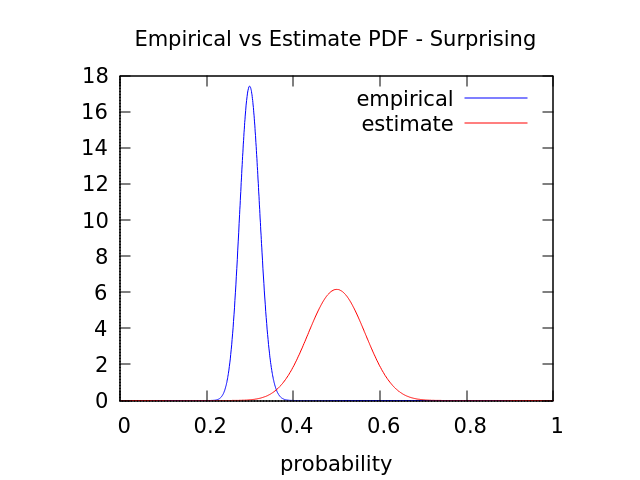
\includegraphics[scale=0.6]{images/surprising.png}
  \end{center}

  - - - - - - - - - - - - - - - - - - - - - - - - - - - - - - - - - -
  - - - - - - - - - - - - - - - - - - - - - - - - - - - - - - - - -\\[0.1cm]
  \center{Download docker image: \texttt{\textcolor{black}{sudo docker pull ngeiswei/opencog:agi20}}}

\end{frame}

\subsection{Surprisingness as reasoning}

\begin{frame}
  % \frametitle{Mining Surprising Patterns as Reasoning}

%%%%%%%%%%%%
%% Speech %%
%%%%%%%%%%%%
  
%% OK, so let me run you through that. The surprisingness is defined
%% as the distance between the empirical distribution and the estimate
%% distribution, here the distance is the Jensen-Shannon distance, so
%% to calculate it you need to infer the empirical distribution, this
%% is easy you just run the pattern over the dataset and counts how
%% many time its true relative to the total size of the dataset. The
%% question is how do you infer the estimate, well the answer is
%% anything, maybe something simple, maybe something very complicated
%% that approximates some type of Solomonoff induction. For now, as
%% currently implemented, we just have one hardwired rule, called IS,
%% which stands for Independence Based Surprisingness Estimate,
%% meaning basically that if the pattern is built up as the
%% conjunction of sub-components we assume these components to be
%% independent. Pretty basic.

%% What we would want though is to have any rule of probability theory
%% and logic allowed, except of course DE, the rule for inferring the
%% empirical distribution, and also to be able to use any background
%% knowledge that may relate to that pattern. If we do that, then we
%% can see that the empirical distributions of other patterns
%% previously considered for surprisingness evaluation can be used,
%% since their empirical distribution is necessary to established
%% their surprisingness, and thus will be part of the knowledge based,
%% therefor could be subsequently used. So for instance, let say we
%% want to infer the surprisingness of a pattern involving white cats,
%% and we already have established the surprisingness of an
%% abstraction of it, say the same pattern over cats in general, as
%% opposed to just white cats, and let say such abstraction is very
%% surprising, we obviously already have its empirical distribution,
%% and this could be combined with other rules to obtain a possibly
%% much better estimate of its specialization, thus decreasing this
%% surprisingness, than it would have been obtained from say an
%% independence based type rule that might have given the high
%% surprisingness over the abstraction, and that would have given the
%% same high surprisingness over the white cat specialization. So we
%% can see that such approach naturally leads to a dynamic measure of
%% surprisingness.

%%%%%%%%%%%%%
%% ~Speech %%
%%%%%%%%%%%%%
  
  \only<1>{
    {\small
      \begin{prooftree}
        \AxiomC{$S \leq \texttt{support}(P, \mathcal{D})$}

        \AxiomC{$P$}
        \AxiomC{$\mathcal{D}$}
        \RightLabel{(DE)}
        \BinaryInfC{$\texttt{emp}(P,\mathcal{D})$}

        \AxiomC{\alert{?}}
        \UnaryInfC{$\texttt{est}(P,\mathcal{D})$}

        \RightLabel{(JSD)}
        \BinaryInfC{$\texttt{jsd}(P,\mathcal{D}))$}

        \RightLabel{(S)}
        \BinaryInfC{$\texttt{surprising}(P, \mathcal{D}, \texttt{jsd}(P,\mathcal{D}))$}
      \end{prooftree}
    }
  }

  \only<2>{
    {\small
      \begin{prooftree}
        \AxiomC{$S \leq \texttt{support}(P, \mathcal{D})$}

        \AxiomC{$P$}
        \AxiomC{$\mathcal{D}$}
        \RightLabel{(DE)}
        \BinaryInfC{$\texttt{emp}(P,\mathcal{D})$}

        \AxiomC{\alert{$P$}}
        \AxiomC{\alert{$\mathcal{D}$}}
        \RightLabel{\alert{(IS)}}
        \BinaryInfC{$\texttt{est}(P,\mathcal{D})$}

        \RightLabel{(JSD)}
        \BinaryInfC{$\texttt{jsd}(P,\mathcal{D}))$}

        \RightLabel{(S)}
        \BinaryInfC{$\texttt{surprising}(P, \mathcal{D}, \texttt{jsd}(P,\mathcal{D}))$}
      \end{prooftree}
    }
  }

  \only<3>{
    {\small
      \begin{prooftree}
        \AxiomC{$S \leq \texttt{support}(P, \mathcal{D})$}
        
        \AxiomC{$P$}
        \AxiomC{$\mathcal{D}$}
        \RightLabel{(DE)}
        \BinaryInfC{$\texttt{emp}(P,\mathcal{D})$}

        \AxiomC{\alert{$\vdots$}}
        \AxiomC{\alert{$\vdots$}}
        \BinaryInfC{\alert{$\vdots$}}
        \AxiomC{\alert{$\vdots$}}
        \BinaryInfC{$\texttt{est}(P,\mathcal{D})$}

        \RightLabel{(JSD)}
        \BinaryInfC{$\texttt{jsd}(P,\mathcal{D}))$}
        
        \RightLabel{(S)}
        \BinaryInfC{$\texttt{surprising}(P, \mathcal{D}, \texttt{jsd}(P,\mathcal{D}))$}
      \end{prooftree}
    }
  }

  \only<4->{
    {\footnotesize
      \begin{prooftree}
        \AxiomC{$S \leq \texttt{support}(P, \mathcal{D})$}
        
        \AxiomC{$P$}
        \AxiomC{$\mathcal{D}$}
        \RightLabel{(DE)}
        \BinaryInfC{$\texttt{emp}(P,\mathcal{D})$}
        
        \AxiomC{\alert{$\texttt{emp}(Q,\mathcal{D})$}}
        \UnaryInfC{\alert{$\vdots$}}
        \AxiomC{\alert{$\vdots$}}
        \BinaryInfC{\alert{$\vdots$}}
        \AxiomC{\alert{$\vdots$}}
        \BinaryInfC{$\texttt{est}(P,\mathcal{D})$}

        \RightLabel{(JSD)}
        \BinaryInfC{$\texttt{jsd}(P,\mathcal{D}))$}
        
        \RightLabel{(S)}
        \BinaryInfC{$\texttt{surprising}(P, \mathcal{D}, \texttt{jsd}(P,\mathcal{D}))$}
      \end{prooftree}
    }
  }

  \visible<5>{\textcolor{white}{\noindent\makebox[\linewidth]{\rule{10cm}{0.4pt}}}}
  
  \only<1-2>{\visible<1>{\begin{center}\alert{ }\end{center}}}
  \only<1-3>{\visible<1>{\begin{center}\alert{ }\end{center}}}
  \visible<5>{\begin{center}\alert{ }\end{center}}

  - - - - - - - - - - - - - - - - - - - - - - - - - - - - - - - - - -
  - - - - - - - - - - - - - - - - - - - - - - - - - - - - - - - - -\\[0.1cm]
  \center{Download docker image: \texttt{\textcolor{black}{sudo docker pull ngeiswei/opencog:agi20}}}

\end{frame}

\begin{frame}

  \center{Tutorial time}
  
  - - - - - - - - - - - - - - - - - - - - - - - - - - - - - - - - - -
  - - - - - - - - - - - - - - - - - - - - - - - - - - - - - - - - -\\[0.1cm]
  \center{Download docker image: \texttt{\textcolor{black}{sudo docker pull ngeiswei/opencog:agi20}}}

\end{frame}

\end{document}
